\chapter{Specification and Requirements Analysis}
\label{chap:Chapter 2 title}
\section{Introduction}


The success of a project heavily relies on the quality of its initiation. Therefore, the functional study phase is crucial for a successful start to the project. This chapter encompasses requirement specifications, including needs analysis involving stakeholder identification, system use cases, and the textual scenarios associated with these use cases.

\pagebreak

\section{Study and analysis of the current state}

Orange Business Services Morocco has embraced an approach known as CI/CD to efficiently manage the development and delivery of its projects. They utilize the GitLab platform, which facilitates swift creation, compilation, testing, delivery, and deployment of software.

In their existing solution, they have established continuous integration and delivery pipelines using GitLab CI, Nexus, Docker, and Kubernetes. Here's how it operates:

\begin{itemize}
  \item Code management and updates are performed using GitLab. Developers push their code changes to the GitLab repository.
  \item The application is containerized using Docker, a technology enabling the creation of isolated and portable environments for applications.
  \item The GitLab Runner conducts a check to ensure the YAML code is correct and clean. Then, it triggers pipeline steps such as Docker image generation and their submission to the Nexus repository.
  \item Kubernetes, aided by Helm (a package manager for Kubernetes), handles the application deployment across various environments. It follows a "Push" deployment model.
\end{itemize}

This approach enables Orange Business Services Morocco to efficiently manage the development and delivery of their projects by automating processes using GitLab, Docker, Nexus, and Kubernetes. It empowers them to deliver high-quality software more rapidly.

\newpage
\subsection{Criticism of the current state}

While utilizing GitLab accelerates software development and deployment, there's a clear need for enhancements focused on sustainability and reducing environmental impact. An exhaustive study of the existing system was conducted to refine our project's scope and expected functionalities, aiming for a more reliable system than the previous one. Identified areas for improvement include

\begin{itemize}
  \item The current CI/CD approach relies heavily on resource-intensive technologies like Docker and Kubernetes, which contribute to increased energy consumption and carbon emissions.
  \item While effective for streamlining development workflows, the pipelines lack mechanisms for tracking and optimizing energy usage.
  \item Without visibility into the energy consumption and carbon footprint of the Kubernetes cluster, targeted strategies for reducing environmental impact are challenging to implement.
\end{itemize}

\subsection{Functional requirements}
Functional requirements gathering is a crucial step in the project. This stage produces the functional specifications document, during which the expected functionalities are formalized along with all governing management rules.

To address the issues identified in the existing study, the principle is to integrate monitoring tools such as Kepler (\emph{Kubernetes-based Efficient Power Level Exporter}), Prometheus, and Grafana into the CI/CD pipeline. This integration aims to measure the energy consumption and CO$_2$ emissions of Orange’s Kubernetes cluster, providing valuable insights for optimizing Green IT practices within the DevOps workflow.

\subsubsection*{Integration of Monitoring Tools}

The integration of these monitoring tools is essential. Kepler will monitor energy consumption and CO$_2$ emissions, Prometheus will collect and store metrics from Kepler, and Grafana will visualize the collected metrics for better insights. Automating the deployment and configuration of Kepler, Prometheus, and Grafana within the CI/CD pipeline is also a key requirement, ensuring that monitoring is an integral part of the continuous integration and deployment processes.

\subsubsection*{GitLab Template Creation}

Creating a GitLab template for GitLab CI/CD pipelines will streamline the process of integrating and deploying Kepler, Prometheus, and Grafana configurations. This template will include automated steps for deployment, configuration, and monitoring setup, ensuring consistency and efficiency across projects.


\subsubsection*{Data Collection and Visualization}

Collecting real-time data on energy consumption and CO$_2$ emissions from the Kubernetes cluster is critical, along with storing historical data for trend analysis and reporting. This data will be visualized using Grafana dashboards, providing customizable views to monitor both real-time and historical data.

\subsubsection*{Alerting and Notification}

Additionally, setting up alerting rules in Prometheus to monitor key metrics such as high energy consumption or CO$_2$ emission levels is vital. Defining thresholds for these alerts will trigger notifications based on predefined conditions.

Integrating Prometheus Alertmanager with Slack to send notifications ensures that alerts are promptly sent to specific Slack channels or user groups for immediate action. This notification system will help in taking timely measures to address any issues related to energy consumption and emissions, thereby supporting the goal of optimizing Green IT practices within the DevOps workflow.



\subsection{Non-Functional requirements}

Non-functional requirements play a crucial role in system design,
because they define the attributes, constraints and restrictions to be taken into account.

These requirements, also called system qualities, guarantee the
user-friendliness and overall efficiency of the system. If any of these requirements are not met,
the system risks not meeting the internal needs of the company, users
or the market.

\begin{itemize}
  \item \textbf{Accuracy}: The system must provide accurate measurements of energy consumption and CO$_2$ emissions to support informed decision-making.
  \item \textbf{Scalability}: Ensure scalability to handle increasing data volumes as the size of the Kubernetes cluster grows.
  \item \textbf{Reliability}: The solution should be reliable, with minimal downtime, to maintain continuous monitoring and data collection.
  \item \textbf{Security}: Implement robust security measures to safeguard sensitive energy consumption and emission data from unauthorized access or tampering.
  \item \textbf{Performance}: Ensure efficient performance to deliver timely insights and visualizations, even during peak usage periods.
  \item \textbf{Ease of Use}: Design an intuitive user interface that allows administrators to easily configure monitoring settings and interpret data visualizations.
  \item \textbf{Compatibility}: Ensure compatibility with existing infrastructure and tools used within Orange Business Services Morocco, such as Prometheus, Grafana, and Kepler.
\end{itemize}


\section{DevOps}
\subsection{Definition}

The word DevOps is a combination of the terms development and operations, meant to represent a collaborative or shared approach to the tasks performed by a company's application development and IT operations teams.
The DevOps methodology aims to shorten the systems development lifecycle and provide continuous delivery with high software quality. These characteristics help ensure a culture of building, testing, and releasing software that is more reliable and at a high velocity.

\subsection{CI/CD}
\textit{Continuous Integration (CI)} is a software development practice where developers frequently merge their code changes into a central repository, typically multiple times a day. Each merge triggers an automated build and testing process. The primary goal of CI is to detect and address issues early in the development cycle, which helps in maintaining code quality and reducing integration problems. By integrating frequently, developers can identify bugs early, facilitating easier and quicker fixes.

\textit{Continuous Delivery (CD)} extends CI by automatically preparing code changes for a release to production. It ensures that the software can be reliably released at any time, with the deployment process being automated but requiring manual approval. Continuous Deployment is a further extension of CD where every change that passes all stages of the production pipeline is automatically released to customers without human intervention. This practice reduces the lead time for delivering new features and fixes, thus providing rapid feedback to developers and stakeholders.


\subsection{Green DevOps:}
Green DevOps extends DevOps principles, focusing on resource efficiency while staying agile. It emphasizes sustainability, reducing environmental impact, and integrating eco-friendly strategies into software development. The goal is to balance technological innovation with ecological responsibility.
\begin{figure}[H]
  \centering
  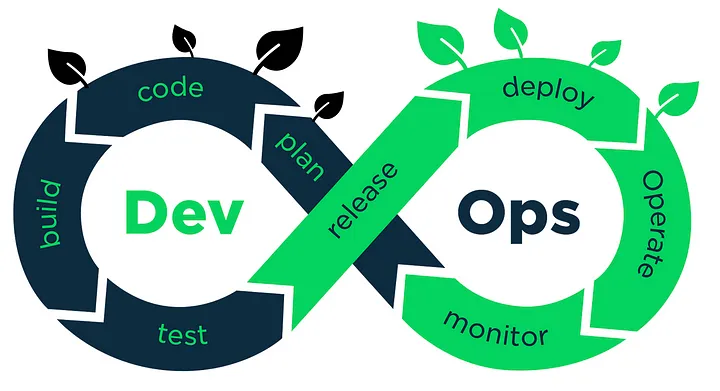
\includegraphics[width=16cm]{Figures/devgreenops.png}
  \caption{Green DevOps}
\end{figure}
\subsection*{The Fundamental Principles of Green DevOps}
Green DevOps is nothing more than an extension of DevOps. It shouldn't be viewed as an upheaval of all DevOps principles. We retain all DevOps principles but adjust them as finely as possible to optimize resource usage.

Green DevOps relies on the following concepts:
\begin{itemize}
  \item \textbf{Infrastructure Optimization:} Choosing eco-friendly data centers, energy-efficient hardware, and effective resource utilization are pillars of Green DevOps. The goal is to reduce energy consumption while maintaining performance.
  
  \item \textbf{Reduction of E-waste:} This involves minimizing over-provisioning of IT resources, properly managing electronic waste, and promoting hardware component recycling.
  
  \item \textbf{Automation and Process Optimization:} Automation is at the core of DevOps, but it holds even greater importance in the context of Green DevOps. Automating tasks reduces energy consumption by minimizing unused resources and enabling fine-grained resource management.
  
  \item \textbf{Carbon Impact Assessment:} To truly become "green," measurement is necessary. Green DevOps integrates tools and metrics to continuously assess and monitor the carbon footprint of projects. This helps identify areas needing improvement and track progress.
  
  \item \textbf{Reduction of Cycle Times:} Shorter development cycles mean less energy consumption and faster time to market. By reducing delays, Green DevOps contributes to the competitiveness of the business while minimizing its environmental impact.
  
  \item \textbf{Awareness:} DevOps teams need to be aware of environmental issues. Employee training and engagement are essential to fostering the adoption of sustainable practices.
\end{itemize}

\subsection*{The Benefits of Green DevOps}

\begin{itemize}
  \item \textbf{Cost Reduction}: Less wasted resources, time saved, and efficient resource utilization result in a significant reduction in operating and infrastructure costs.
  
  \item \textbf{Quality Improvement}: Green DevOps practices encourage automation, monitoring, and rigorous testing, leading to better software quality, fewer bugs, and an enhanced user experience.
  
  \item \textbf{Social Responsibility}: Companies adopting Green DevOps demonstrate their commitment to environmental sustainability, which can enhance their brand image and attract new customers and talents.
  
  \item \textbf{Regulatory Compliance}: With an increasing number of environmental regulations in place, Green DevOps helps companies comply with standards and avoid potential penalties.
\end{itemize}

\subsection{DevOps Monitoring}
DevOps monitoring is the process of tracking and measuring the performance of applications and systems in order to help software development teams identify and resolve potential issues more quickly. This is typically done via a manual or automated DevOps monitoring solution or a collection of continuous monitoring tools that gather data

\subsection*{DevOps Monitoring Use Cases}

The main benefit of DevOps monitoring is its ability to define, track, and measure KPIs across all aspects of DevOps. Here are some specific use cases of DevOps monitoring:

\begin{itemize}
  \item \textbf{Detect and Report Errors Earlier:}
  Flagging issues to DevOps teams more quickly means they can resolve them before they impact user experience. Early detection and reporting of errors allow for prompt resolution, minimizing disruptions and maintaining a smooth user experience.
  \item \textbf{Reduce System Downtime:}
  DevOps monitoring tools provide continuous oversight of databases, applications, and networks, enabling teams to resolve issues before system downtimes occur. By proactively identifying potential problems, teams can take preemptive actions to avoid outages and ensure system reliability.
  \item \textbf{Enhance Observability of DevOps Components:}
  Easily identify when various systems and applications in your DevOps stack degrade in performance, cost, security, or other factors to avoid problems down the road. Enhanced observability enables teams to maintain optimal performance and security by monitoring and analyzing system behavior continuously.

  \item \textbf{Uncover Root Cause of Issues Faster:}
  Continuous tracking of logs and metrics helps teams identify the root cause — where a problem started or occurred. This allows engineers to detect patterns in system behavior to anticipate and prevent future issues, improving mean time to detection (MTTD), mean time to repair (MTTR), and mean time to isolate (MTTI).
\end{itemize}



\section{Benchmark}

\subsection{Scaphandre vs. Kepler}

In the landscape of power consumption monitoring tools, Scaphandre and Kepler stand out as prominent contenders. As organizations increasingly prioritize energy efficiency and sustainability, understanding the capabilities of these tools becomes crucial. In this benchmark, we compare Scaphandre and Kepler to provide insights into their strengths and suitability for diverse computing environments.

\begin{table}[htbp]
  \centering
  \begin{tabular}{|p{3cm}|p{6cm}|p{6cm}|}
  \hline
  \textbf{Aspect} & \textbf{Scaphandre} & \textbf{Kepler} \\
  \hline
  Scope and Granularity & Provides per-process power usage monitoring. Collects real-time power consumption metrics from system components using sensors like RAPL. & Offers estimation of power consumption at the process, container, and Kubernetes pod levels. Utilizes various APIs and sensors to collect real-time power metrics, including RAPL for CPUs and DRAM, NVML for GPUs, ACPI for platform power, etc. \\
  \hline
  Environment Support & Primarily focused on monitoring power consumption in the host environment. & Supports both bare-metal and virtualized environments. Provides ways to estimate power consumption in VMs on public clouds where direct power metrics may not be available. \\
  \hline
  Modeling and Estimation & Utilizes a ratio-based model to estimate power consumption per process based on resource utilization metrics collected from the system. Relies on sensors like RAPL to measure absolute power consumption. & Employs various models, including trained power models for VMs in public clouds and regression-based models, to estimate power consumption at different levels within the environment. \\
  \hline
  Training and Optimization & Does not involve explicit training of power models. Relies on direct sensor readings and resource utilization metrics to estimate power consumption. & Includes a Model Server component for training power models using Prometheus metrics from bare-metal nodes. The models are continuously optimized for accuracy and can be shared publicly for use in various environments. \\
  \hline
  Limitations and Future Enhancements & Acknowledges limitations such as the accuracy of pre-trained power models, challenges in estimating power in virtualized environments, and overhead issues. & Acknowledges similar limitations and actively works on enhancements, including broader support for power data sources, vendor-agnostic support, performance optimization, and multi-level deployment strategies for accurate power estimation in VMs. \\
  \hline
  \multicolumn{3}{|p{15cm}|}{\textbf{Best Choice:} Kepler stands out as the best choice due to its comprehensive approach to power consumption monitoring and estimation. With support for multiple environments, advanced modeling techniques, continuous optimization of power models, and active development for future enhancements, Kepler offers a robust solution for accurate and efficient power management in modern computing environments.} \\
  \hline
  \end{tabular}
  \caption{Comparison of Scaphandre and Kepler}
  \label{tab:comparison}
  \end{table}

\subsection{Kepler}

\begin{figure}[H]
  \centering
  
\includegraphics[width=10cm]{Logos/kepler-logo.png}
  \caption[]{Kepler-logo}
\end{figure}
Kepler, short for Kubernetes-based Efficient Power Level Exporter, is a sophisticated tool designed to measure and estimate power consumption at various levels within a cloud infrastructure. It aims to provide detailed insights into the energy usage of processes, containers, and Kubernetes pods, making it an invaluable resource for both industrial and research projects. Kepler’s architecture is extensible, allowing for the integration of novel power models that cater to diverse system architectures. This tool is essential in an era where efficient energy consumption is critical to minimize environmental impact and manage operational costs effectively.

\subsection{Kepler Functionalities}

Kepler offers several key functionalities that make it a powerful tool for monitoring and optimizing energy consumption in cloud environments:

\begin{enumerate}
    \item \textbf{Real-Time Power Metrics Collection:} Kepler can gather real-time power consumption metrics from various hardware components, such as CPUs, GPUs, and DRAM. This is achieved through the use of APIs like Intel Running Average Power Limit (RAPL) and NVIDIA Management Library (NVML). These metrics provide an accurate and immediate view of the power usage of different system components.

    \item \textbf{Power Consumption Estimation:} Kepler estimates power usage at multiple levels, including processes, containers, and Kubernetes pods. By analyzing resource utilization metrics, Kepler can determine the energy consumption of individual components and aggregate these to provide a comprehensive view of the system's power usage. This granular estimation is crucial for identifying power-hungry processes and optimizing resource allocation.

    \item \textbf{Extensible Power Models:} One of Kepler's strengths is its extensibility. It allows for the integration of custom power models, which can be tailored to different system architectures and hardware setups. This adaptability ensures that Kepler can provide accurate power consumption estimates across a variety of environments, making it a versatile tool for both industrial and research applications.

    \item \textbf{Data Aggregation and Storage:} The power consumption data collected and estimated by Kepler are stored in Prometheus, a powerful monitoring and alerting toolkit. This integration facilitates easy access, analysis, and visualization of power metrics. Users can query Prometheus to gain insights into energy consumption patterns and identify opportunities for optimization.

    \item \textbf{Support for Bare-metal and Virtual Machines:} Kepler is designed to operate in both bare-metal and virtual machine (VM) environments. In bare-metal nodes, it uses direct power metrics from hardware components. In VM environments, where direct power metrics are not available, Kepler employs trained power models to estimate power consumption. This dual approach ensures that Kepler can provide valuable insights regardless of the underlying infrastructure.
\end{enumerate}

\subsection{How Kepler collects metrics?}
The method for collecting system power consumption metrics in Kepler varies based on the deployment environment—bare-metal (BM) or virtual machines (VMs).

In bare-metal environments, Kepler directly collects real-time system power metrics and utilizes the Ratio Power model to estimate power consumption. This model splits the dynamic power (related to resource utilization) proportionally across processes, while idle power (constant regardless of load) is divided according to the size of processes/containers as per the GreenHouse Gas (GHG) protocol. Hardware counters are used to assess CPU, memory, and GPU utilization.

In public cloud VM environments, direct power measurement isn't feasible. Instead, Kepler uses trained power models for estimation. These models are based on regression analysis of data from benchmark tests. Kepler can also help cloud providers expose VM power metrics by measuring power at the BM level and passing this data to VMs via hypervisor Hypercalls. Within VMs, Kepler applies the Ratio Power Model to estimate power usage per process, using eBPF metrics due to the absence of hardware counters. However, Kepler does not estimate idle power for VMs due to unknowns about other running VMs on the host.

The trained power models allow for accurate power estimation despite the limitations of VM environments, and Kepler's approach ensures adaptability across different deployment scenarios.


\begin{figure}[H]
  \centering
  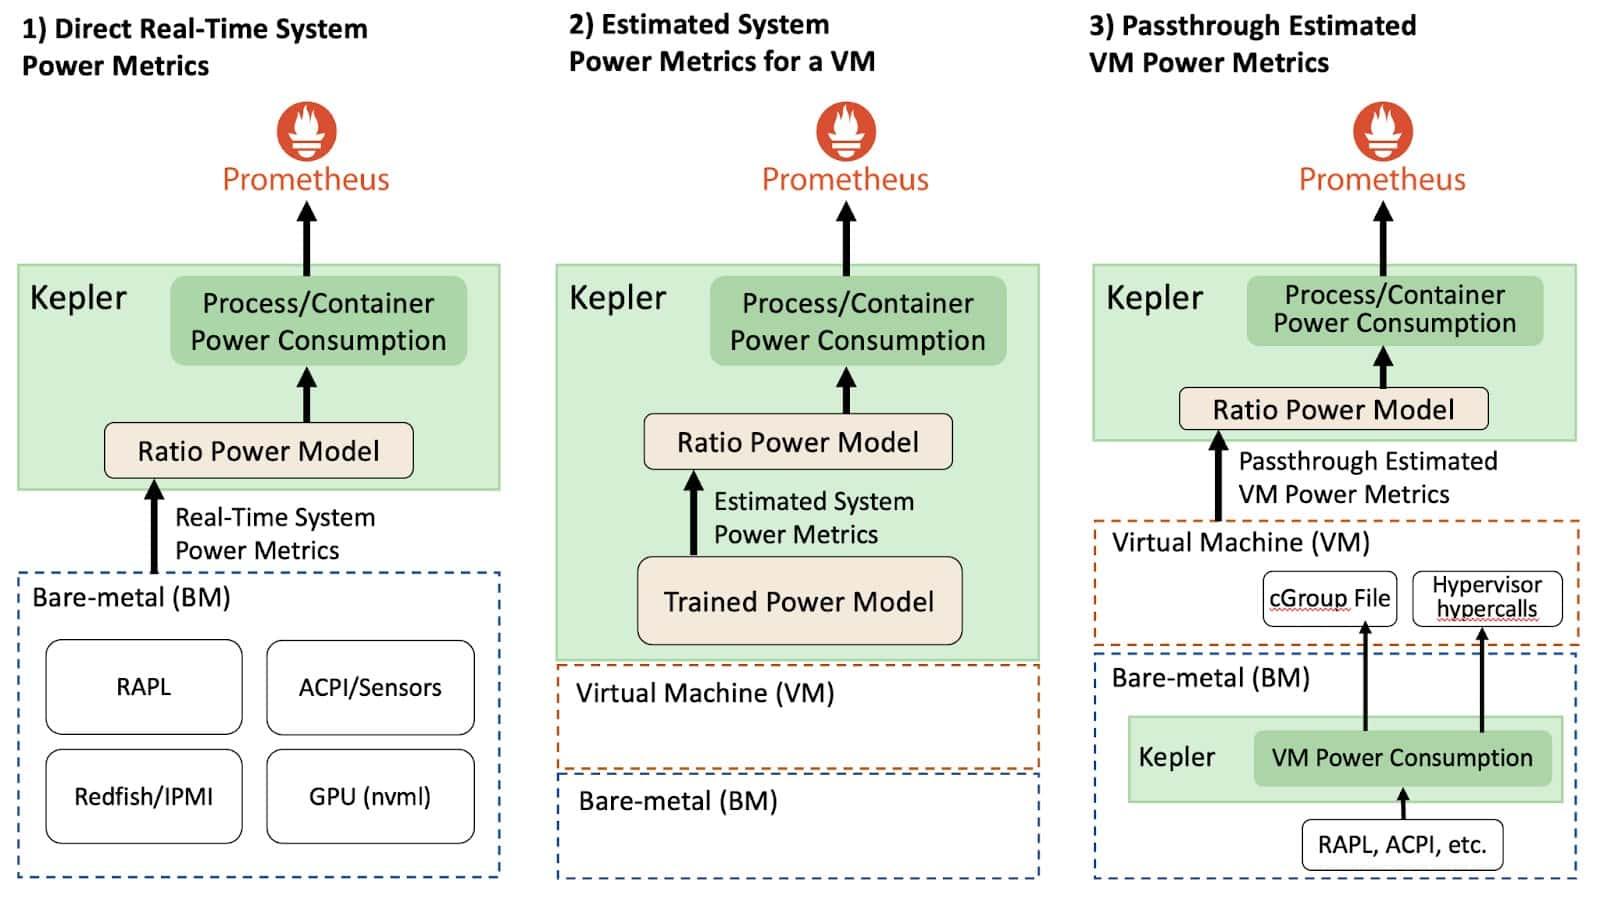
\includegraphics[width=16cm]{Figures/kepler-system-power-consumption.jpg}
  \caption{Collecting System Power Consumption – VMs versus BMs}
\end{figure}



\newpage


\section{Identification of Stakeholders}
\label{subsec:identification_stakeholders}

Identifying stakeholders is a fundamental step in any development project. It helps to understand the interactions and measure the influence of each group on the actions to be undertaken. But what exactly is a stakeholder? A stakeholder can be a physical person or a legal entity that participates in or is affected by the action or project in question. It is important to clearly specify the action or series of actions for which we seek to determine who the stakeholders are and what they represent.

In the context of integrating Green IT into DevOps practices at Orange Business Services Morocco, we identify the following stakeholders:

\begin{itemize}
  \item \textbf{Platform Admin Team}: Responsible for setting up staging and production environments, managing cluster extension modules, and other cluster resources (controllers and admission webhooks), integrating development team repositories using customized GitRepository resources, and configuring how development team repositories are reconciled on each cluster.
  
  \item \textbf{Development Team}: Configures application definitions at the Kubernetes deployment level, manages Helm releases, configures how applications are reconciled across environments, and oversees the promotion of applications between environments.
  
  \item \textbf{Green IT Team}: Responsible for analyzing the energy consumption and CO$_2$ emissions of the Kubernetes clusters. 
  
  \item \textbf{GitLab}: A secondary stakeholder that manages team access and coordinates the CI/CD processes.
\end{itemize}

By identifying these stakeholders and their respective roles, we can ensure a comprehensive approach to integrating Green IT into our DevOps practices, balancing rapid software delivery with environmental responsibility.


\section{Conclusion}

This chapter outlined the essential functional and non-functional requirements for integrating monitoring tools into the CI/CD pipeline. By leveraging Kepler, Prometheus, and Grafana, we aim to provide accurate, scalable, and reliable measurements of energy consumption and CO$_2$ emissions. Emphasis was placed on security, performance, ease of use, and compatibility with existing infrastructure. These requirements form the blueprint for implementation, ensuring the system meets its objectives and supports informed decision-making through effective monitoring and visualization.



















